\documentclass{tufte-handout}
\usepackage{amsmath,amsthm}

\input{vc.tex}

\usepackage{pgfplots}
\pgfplotsset{width=\textwidth,compat=1.5.1}

\newtheorem{claim}{Claim}[section]
\title{\sf Pagerank}
%\date{\GITAuthorDate}
%\author{Thore Husfeldt}

\begin{document}
\maketitle
\footnotetext{rev. \GITAbrHash}

\section{Pagerank}
Consider an directed multigraph $G=(V,E)$ without self-loops, as in
Fig.~1.
We will understand $G$ as the hyperlink structure of the web pages
described by $V$; an an arc from vertex $u$ to vertex $v$ describes a
hyperlink from page $u$ to page $v$.

The \emph{random surfer} model is a stochastic process that aims to
rank the relevance of a these pages.
The states of this process are the vertices $V$.
With good probability $\alpha$, the process picks an outgoing edge at
random and moves to that page.
(Note that outgoing edges are counted with multiplicities, so from
vertex~1 in the example, the chance of going to 3 is double that of
going to 4.)
Alternatively, with probability $(1-\alpha)$, the surfer becomes bored
and moves to a random page from $V$ instead.

This process is a Markov chain.\sidenote{In fact, a finite,
  irreducible, and ergodic Markov chain, provided $G$ is finite.}
Its stationary distribution describes the \emph{page rank} of each
vertex.

\subsection{Files}

Vertex names are integers $V= \{0,\ldots, n-1\}$.
Input files contain $|V|$, followed by $u$ and $v$ for each $(u,v)\in
E$.

\begin{marginnote}
\begin{verbatim}
3
0 1   0 1   0 2
1 2   
2 0   2 1
\end{verbatim}
\caption{Input file for the graph in Fig.~1.}
\end{marginnote}

The files are
\begin{description}
\item[three.txt] The 3-vertex graph from Fig.~1.
\item[tiny.txt] The 5-vertex graph from \S{}1.6. in [Sedgewick and Wayne,
  \emph{Programming in Java: An Interdisciplinary Approach}, Addison
  Wesley, 2007]
\item[medium.txt] The 50-vertex graph \emph{ibid.}
\item[wikipedia.txt] The 11-vertex graph from
  [``PageRank.'' Wikipedia, The Free Encyclopedia. Wikimedia
  Foundation, Inc. Accessed 16 Sep 2012.]

\end{description}

\subsection{Deliverables}

\begin{enumerate}
\item Implement a simulation of the random surfer model. 
  Start in
  vertex 0 and follow the rules for a given number of iterations read
  from the command line. Count the number of times each vertex is
  visited and print the relative frequencies.
\item Solve the exact same problem using linear algebra instead of
  simulation.
  That is, construct the transition probability matrix $P$ and
  compute $pP^m$ for some sufficiently high $m$ (read from the command
  line).
\item Fill out the report.
\end{enumerate}


\newpage
\section{Maxcut Lab Report}


by Alice Cooper and Bob Marley\sidenote{Complete the report by filling
  in your names and the parts marked $[\ldots]$.
  Remove the sidenotes in your final hand-in.}

\subsection{Running time}

The running time of algorithm~R is $[\ldots]$\sidenote{Replace
  $[\ldots]$ by a function of $n$ and/or $m$. You can use asymptotic
  notation. This is supposed to be easy.}.

\subsection{Randomness}

Algorithm R uses $[\ldots]$\sidenote{Replace
  $[\ldots]$ by a function of $n$ and/or $m$. Do not use asymptotic
  notation. This is supposed to be easy.} random bits.

\subsection{Solution quality}

\paragraph{Experiments.}

\begin{enumerate}
\item
For the input file  pw09\_100.9.txt with $t=100$ runs, we found
an average cutsize of $C=[\ldots]$, roughly $[\ldots]$\% of the optimum
$\operatorname{OPT} = 13658$.
The distribution of cutsizes looks as follows:\sidenote{Display your
  cutsizes as a histogram. Use whatever software you like to produce
  the image; the placeholder image on the left is constructed in the
  \LaTeX\ source.}

\medskip

\noindent
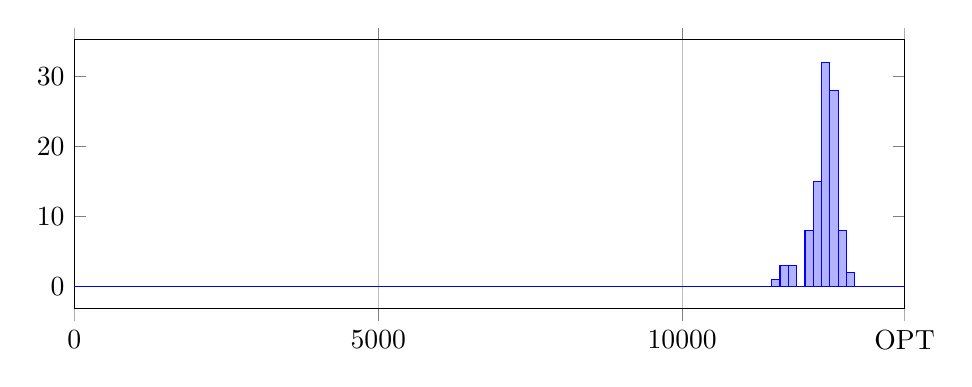
\begin{tikzpicture}
\begin{axis}[
  height= 5cm,
  ybar interval,
  xmin = 0,  xmax = 13658,
  xtick =       {0   ,   5000,   10000, 13658},
  xticklabels = { $0$, $5000$, $10000$,   OPT},
  x tick label as interval = false,
  scaled ticks = false
]
    \addplot+[hist={bins=100}]
        table[y index=0] {
          % output of 
          % perl -e "for $i (1..100) { system 'python sol/rmaxcut.py < data/pw09_100.9.txt '}"
12296
12401
12176
12414
11767
12458
12407
12551
12363
12526
11865
12353
12159
12504
12130
11616
12347
12201
12473
12368
12196
12274
12064
12398
12733
12620
12402
12231
12442
12360
12567
11650
12334
12543
12108
12523
12256
12524
12642
12040
12404
12408
12606
12094
12484
12457
12459
12326
12307
12282
12276
12459
12107
12474
12410
12109
12308
12471
12588
12473
12338
12499
12233
12453
12448
12541
12488
12497
12230
12393
12335
12446
11503
12304
12612
12378
12108
12684
12422
12557
12441
12334
12400
12369
11734
12237
12631
12289
11773
12460
12366
12355
12502
12323
12543
12271
12415
12227
12711
12370
    };
\end{axis}
\end{tikzpicture}

\item
For the input file matching\_1000.txt
$[\ldots]$\sidenote{Perform the same analysis for 
    matching\_1000.txt. This involves thinking to determine OPT.}
\end{enumerate}
\paragraph{Analysis of performance guarantee}

Clearly, Algorithm R performs quite badly on input 
  matching\_1000.txt.
We will show that it can perform \emph{no worse} than that, i.e., we
will establish that in expectation, the cutsize $C$ satisfies $C \geq
[\ldots]\cdot \operatorname{OPT}$.\sidenote{Replace [\ldots] by the
  right constant}


We will view $C$ as a random variable that gives the size of the cut
defined by the random choices.
Let $W$ denote the total weight of the edges of $G$, i.e.,
\[ W= \sum_{e\in E} w(e)\,.\]

Then,
\begin{equation}\label{eq: E[C]}
E[C] = \textstyle\frac{1}{2}\cdot W\,.
\end{equation}

To see this, define the indicator random variable $X_{uv}$ for every
edge $uv\in E$ as follows.
Set $X_{uv}=1$ if $uv$ crosses the cut, i.e., $u\in A$ and $v\notin A$
or $u\notin A$ and $v\in A$.
Otherwise, $X_{uv} = 0$.

Then, $\Pr(X_{uv} = 1) = [\ldots]$.
Now, $E[C]=[\ldots]$ Finally, we have 
\(E[C]\geq [\ldots]\cdot \text{OPT}\) because clearly
$[\ldots]$.\sidenote{Fill in the missing blanks in this paragraph.
  Your calculations and arguments need to include phrases like
  ``because BLA and BLA are independent'' or ``disjoint,'' and ``by
  linearity of expectation'' and ``because the weights are positive.''

}


\newpage
\section{Optional: Derandomising Algorithm R}

\subsection{Algorithm L} 


We now reduce the number of random bits used by the algorithm to $\log
n$ using a simple \emph{pseudorandom generator}.


Let $k=\lceil\log (n+1)\rceil$ and flip $k$ coins $b_1,\ldots, b_k$.
There are $2^k -1 \geq n$ different ways of choosing a nonempty subset
$S\subseteq [k]$ of the coins.
Each of these ways defines a random bit $r_S =\bigoplus_{i\in S} b_i$.
(Here, $\xor$ denotes exclusive or.)
This gives a total of $n$ random bits.
These random bits are not as high-quality as the original $k$ bits,
but they retain the crucial property of \emph{pairwise independence}:
If $S\neq T$ then
\[ \Pr(r_S\neq r_T) = [\ldots],.\]

Extend Algorithm~R using this idea; call the resulting
algorithm~L (for logarithmic randomness).

\subsection{Algorithm Z}

For our final trick, we let the random bits disappear completely:
since Algorithm~L uses only $k$ bits of randomness, we can iterate
over \emph{all} coin flips---there are only $2^k$, which is polynomial
(in fact, linear) in $n$.
Extend algorithm~L using this idea; call the resulting algorithm~Z
(for zero randomness).
The running time of Z is $O([\ldots])$.

\newpage
\section{Perspective}

This lab establishes minimal skills in algorithms implementation,
probabilistic analysis of algorithms (independence, linearity of
expectation, and in particular the trick of computing an expectation
using indicator random variables), and approximation guarantees (in
particular, finding upper and lower bounds by exhibiting a concrete
``bad instance'' and a comparison to a hypothetical optimum,
respectively).
The histogram aims to establish the intuition that measure is
concentrated around its expectation.

\bigskip

To establish that Maxcut is NP-hard one reduces from NAE-Sat, a
reduction that can be found in many places\sidenote{C. Moore and
S. Mertens, \emph{The Nature of Computation}, Oxford University Press,
  2011, p. 146.}
Recall that the related problem \emph{Minimum Cut} is easy because of
the max flow--min cut theorem.
A moment's thought should convince you that as soon as negative
weights are allowed, the two problems are the same (and both are
hard).
Algorithm R doesn't work at all for negative weights.

Algorithm R is a classical randomised approximation algorithm, its
origins seem to be shrouded in the mists of time.
The \emph{deterministic} algorithm of Sahni and Gonzales\sidenote{S.\
  Sahni and T.\ Gonzalez.
  P-complete approximation problems.
  \emph{J.\ Assoc.\ Comput.\ Mach.}, 23(3):555--565, 1976.}
can be viewed as a derandomisation of R using the \emph{method of
  conditional expectations}.
These algorithms were best knows until the breakthrough result of
Goemans and Williamson,\sidenote{M.\ X.\ Goemans and D.\ P.\
  Williamson.
  Improved approximation algorithms for maximum cut and satisfiability
  problems using semidefinite programming.
  \emph{J.\ Assoc.\ Comput.\ Mach.}, 42(6):1115--1145, 1995.}
which improved the approximation factor to $0.87856$.
H\aa{}stad has shown that no algorithm can approximate the maxcut
better than $16/17\sim 0.941176$ unless P equals NP. Khot has shown
that the Goemans--Williamson bound is essentially optimal under the
\emph{Unique Games Conjecture}.

Algorithm L can also be viewed as an application of \emph{pairwise
  independent hash functions}.


\end{document}
